\documentclass{article}
\usepackage{tikz}
\usepackage{float}
\usepackage{amsmath}
\usepackage{lmodern}
\usepackage{amssymb}
\usetikzlibrary{calc}
\usetikzlibrary{hobby}
\usetikzlibrary{decorations.markings}

\begin{document}

\centering

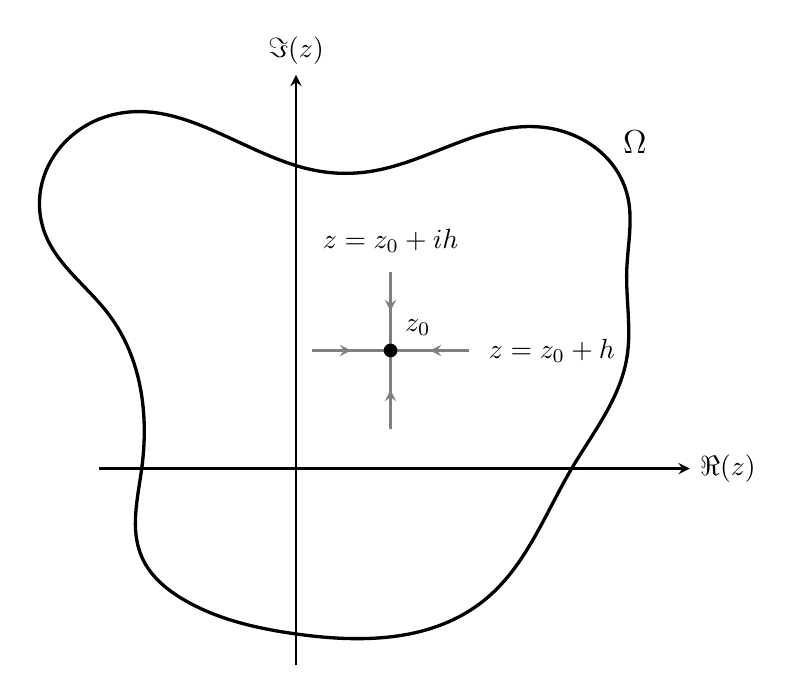
\begin{tikzpicture}
\pgfmathsetmacro{\CircleSize}{0.08}     % radius of coordinate circles/dots
% define styles used in this picture
\tikzset{
BigTextFont/.style={font=\large},
every node/.style={font=\normalsize, text=black},
CircleNodeStyle/.style={draw=black, shape=circle, fill=black, minimum size=\CircleSize*2 cm, inner sep=0pt},
arrowstyle/.style={->, >=stealth}}

%axes
\pgfmathsetmacro{\OvershootAxis}{2.5}
\pgfmathsetmacro{\AxisSize}{5.0} 
\draw[arrowstyle, thick] (-\OvershootAxis,0) -- (\AxisSize,0) node[pos=1, right] {$\Re(z)$};
\draw[arrowstyle, thick] (0,-\OvershootAxis) -- (0,\AxisSize) node[pos=1, above] {$\Im(z)$};

% waypoint coordinates (per quadrant)
\begin{scope}[scale=1.4]
\coordinate (Odegrees) at (2.5,0);
\coordinate (20degrees) at (3,1);
\coordinate (30degrees) at (3,1.8);
\coordinate (40degrees) at (3,2.5);
\coordinate (55degrees) at (2.2,3.1);
\coordinate (80degrees) at (0.7,2.7);
\coordinate (85degrees) at (0.2,2.7);
\coordinate (110degrees) at (-1.7,3.2);
\coordinate (125degrees) at (-2.3,2.2);
\coordinate (130degrees) at (-1.7,1.4);
\coordinate (180degrees) at (-1.4,0);
\coordinate (210degrees) at (-1.4,-0.8);
\coordinate (225degrees) at (-1.0,-1.2);
\coordinate (270degrees) at (0,-1.5);
\coordinate (330degrees) at (1.7,-1.2);
\end{scope}

% CHECK
%plotting the waypoints
%\foreach \c in {(Odegrees),(20degrees),(30degrees),(40degrees),(55degrees),(80degrees),
%(85degrees),(110degrees),(125degrees),(130degrees),(180degrees),(210degrees),(225degrees),(270degrees),(330degrees)} \fill[red] \c circle (0.5mm);

% drawing area ("hobby" package)
\draw[postaction={decorate}, decoration={
       markings,
       mark=at position 0.17 with {\node[above right, BigTextFont] {$\Omega$};}}]
[very thick] (Odegrees) to[closed, curve through =
{ (20degrees) (30degrees) (40degrees) (55degrees) (80degrees) (85degrees) (110degrees) (125degrees) (130degrees)  (180degrees) (210degrees) (225degrees) (270degrees) }] (330degrees);

% Zo coordinate
\coordinate (ZOLocation) at (1.2,1.5);

% Vertical limit
\coordinate (UpperVerticalLimit) at ($(ZOLocation)+(0,1)$);
\coordinate (LowerVerticalLimit) at ($(ZOLocation)+(0,-1)$);
\draw[postaction={decorate}, decoration={
       markings,
       mark=at position 0.50 with {\arrow{stealth}}}]
[gray, thick] (UpperVerticalLimit) -- (ZOLocation);
\draw[postaction={decorate}, decoration={
       markings,
       mark=at position 0.50 with {\arrow{stealth}}}]
[gray, thick] (LowerVerticalLimit) -- (ZOLocation);
\node [label=above:{$z=z_{0}+ih$}] at (UpperVerticalLimit) {};

% Horizontal limit
\coordinate (UpperHorizontalLimit) at ($(ZOLocation)+(1,0)$);
\coordinate (LowerHorizontalLimit) at ($(ZOLocation)+(-1,0)$);
\draw[postaction={decorate}, decoration={
       markings,
       mark=at position 0.50 with {\arrow{stealth}}}]
[gray, thick] (UpperHorizontalLimit) -- (ZOLocation);
\draw[postaction={decorate}, decoration={
       markings,
       mark=at position 0.50 with {\arrow{stealth}}}]
[gray, thick] (LowerHorizontalLimit) -- (ZOLocation);
\node [label=right:{$z=z_{0}+h$}] at (UpperHorizontalLimit) {};

% z0 point
\node [CircleNodeStyle, label=above right:$z_{0}$] at (ZOLocation) {};

\end{tikzpicture}

\end{document}